\documentclass[utf8,usehyperref,12pt]{G7-32}
\input glyphtounicode.tex                   % Нужно для
\pdfgentounicode=1                          % поиска по pdf в кириллице
\usepackage[T2A]{fontenc}
\usepackage{pscyr}
\usepackage[utf8]{inputenc}                 % ваша любимая кодировка здесь
\usepackage[english,russian]{babel}         % это необходимо для включения переносов
\usepackage{float}
\usepackage[pdftex]{graphicx}
\usepackage{array}
\usepackage{mversion}                       % Версионирование
\TableInChaper                              % таблицы будут нумероваться в пределах раздела
\PicInChaper                                % рисунки будут нумероваться в пределах раздела
\setlength\GostItemGap{2mm}                 % для красоты можно менять от 0мм
\sloppy                                     % переносы

\newcounter{MinoreCounter}                  % Новый счетчик минорных версий
\setcounter{MinoreCounter}{1}               % Текущая минорная версия

\renewcommand{\theequation}{(\arabic{chapter}.\arabic{equation})}   % Формат нумерации формул "Глава.номер"
\renewcommand{\version}{\versionnumber.\theMinoreCounter.\thebuildcounter} % Формат версии

\makeatletter
\@addtoreset{equation}{chapter}             % Счетчик формул
\makeatother

\setcounter{page}{3}                        % Начало нумерации страниц
\setVersion{3}                              % Текущая мажорная версия
\increaseBuild                              % Увеличивать номер сборки при каждой компиляции
%<------------- НАЧАЛО ДОКУМЕНТА ---------------------------


\begin{document}
\tableofcontents

\begin{center}
Текущая версия документа: \version~от \today 
\end{center}

\chapter{Работа \No1. Знакомство со средой разработки IAR Embedded Workbench for ARM (EWARM). Разработка программы с использованием библиотеки Standard Peripherals Library (SPL)}
Цель работы: 
\begin{itemize}
\item Знакомство со средой разработки IAR.
\item Изучение принципов работы со светодиодами, знакомство со Standard Peripherals Library (SPL).
\item Изучение принципов отладки программы в среде IAR.
\end{itemize}
\section{Обзор платы STM32L-Discovery}
В данной работе используется отладочная плата STM32L - Discovery на базе 32 МГц микроконтроллера STM32L152RB с 128 KБ Flash, 16 KБ RAM и 4 KБ EEPROM от STMicroelectronics.  Микроконтроллер построен на основе ядра Cortex-M3. Данные микроконтроллеры отличаются ультранизким энергопотреблением (порядка 270 нА в спящем режиме). STM32L-Discovery --- полноценный инструментарий, включающий в себя отладочную плату, программатор и отладчик с поддержкой самых популярных программных средств разработки от таких фирм как IAR, Keil и Atollic. Сигналы встроенного программатора-отладчика ST-Link выведены на внешний разъем, что позволяет в дальнейшем использовать STM32L-Discovery в качестве программатора-отладчика для своих собственных разработок.

Основные характеристики STM32L-Discovery:
\begin{itemize}
\item Микроконтроллер STM32L152RBT6
\item Ядро Cortex-M3, 128 KB Flash, 16 KB RAM, 4 KB EEPROM
\item Интерфейсы USB 2.0 FS, 3xUSART, 2xSPI, 2xI2C, 8 таймеров
\item 24-канальный 12-бит АЦП, компараторы, 2х12-бит ЦАП
\item Полноценные часы реального времени
\item Встроенный контроллер LCD 8х40
\item Встроенный программатор ST-Link с возможностью программировать другие микроконтроллеры STM32.
\item LCD дисплей 24х8 в форм-факторе DIP28
\item Возможность измерения потребляемого тока
\item Четыре светодиода:
\begin{itemize}
\item LD1 (красный/зеленый) для сигнализации обмена данных по USB
\item LD2 (красный) для питания 3.3В
\item Два пользовательских диода LD3 (зеленый) и LD4 (синий)
\end{itemize}
\item Две кнопки (user и reset)
\item Сенсорная клавиатура (четыре сенсорных кнопки или один слайдер)
\item Все свободные выводы STM32L152RBT6 выведены на контактные площадки
\end{itemize}

Летом 2013 года появилась отладочная плата STM32L152C-DISCO из линейки DISCOVERY на базе микроконтроллера STM32L152RCT6, который отличается от STM32L152RB большим объемом памяти: 256 КБ Flash-памяти, 32 КБ ОЗУ и 8 КБ EEPROM.



\section{Общие сведения о ядре Cortex}

Семейство ARM Cortex --- новое поколение процессоров, которые выполнены по стандартной архитектуре. В отличие от других процессоров ARM, семейство Cortex является завершенным процессорным ядром. 

Семейство Cortex доступно в трех основных профилях: 
\begin{itemize}
\item \textit{Cortex-A} --- для высокопроизводительных применений. Это полноценные процессоры общего назначения для самых различных задач. Процессор Apple A5, используемый в iPhone 4S и iPad 2, построен на основе ядра Cortex-A9.
\item \textit{Cortex-R} --- профиль для операционных систем реального времени (ОСРВ, англ. Real-Time Operating System).
\item \textit{Cortex-M} --- для чувствительных к стоимости и микроконтроллерных применений. 
\end{itemize}

Для упрощение разработки под микроконтроллер используется \textit{CMSIS (Cortex Microcontroller Software Interface Standard)}. \textit{CMSIS} --- уровень абстракции аппаратного обеспечения для Cortex-M, обеспечивающий последовательный и простой интерфейс программного обеспечения для процессора и периферийных устройств. \textit{CMSIS} стандартизирует программное обеспечение, позволяя переносить его на другие устройства Cortex-M. 

CMSIS состоит из нескольких файлов:
\begin{itemize}
\item \textit{core\_cm3.c, core\_cm3.h}\footnote{IAR, начиная с версии 6.2, использует собственные файлы core\_cm3.c, core\_cm3.h} --- описание ядра, стандартизировано для всех Cortex-M3.
\item \textit{stm32l1xx.h} --- файл описание периферии, а также структуры доступа к ним. 
\item \textit{system\_stm32l1xx.c} --- функции CMSIS. 
\item \textit{system\_stm32l1xx.h} --- заголовочные файлы для функций CMSIS.
\end{itemize}

CMSIS доступен на сайте производителя микроконтроллеров.


\section{Создание проекта в IAR}

IAR EWARM --- интегрированная среда разработки, включающая в себя компилятор языка Си, отладчик (debugger) и компоновщик (linker). Создание программного обеспечения для микроконтроллера подразумевает создание проекта, который будет объединять CMSIS, сторонние библиотеки и исходные коды на языке Си. Для создание нового проекта нужно выбрать:
\begin{center}
\textit{Project => Create New Project}
\end{center}


\begin{figure}[h!]
\begin{center}
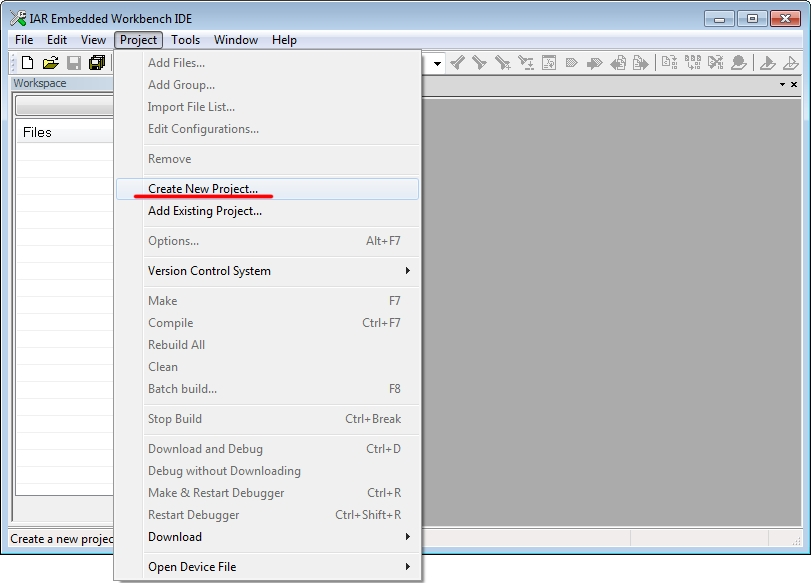
\includegraphics[scale=0.5]{Image/4_1}
\end{center}
\caption{Создание нового проекта}
\end{figure}

В появившемся окне можно выбрать язык программирования. В данной лабораторной это язык Си. Подпункт \textit main позволяет создать файл главной программы \textit{main.c} вместе с каркасом функции \verb\main()\.

\begin{verbatim}
int main()
{
  return 0;
}
\end{verbatim}



\begin{figure}[h!]
\begin{center}
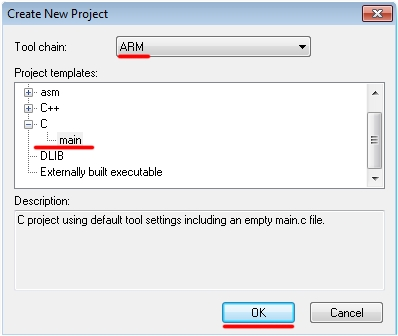
\includegraphics[scale=0.6]{Image/5.jpg}
\end{center}
\caption{Выбор языка программирования}
\end{figure}


Файлы внутри проекта можно объединять в группы (папки, подпапки).  Для упрощения работы с периферией существуют библиотеки \textit{Standard Peripherals Library (SPL)}. В данной работе потребуются библиотека для работы с \textit{GPIO (General Purpose Input-utput)} -- портами ввода-вывода общего назначения и библиотека для работы с \textit{RCC (Reset and Clock Control)} -- системой тактирования и сброса. Создайте группу \textit{SrdPereph}, в ней подпапки \textit{inc} -- для заголовочных файлов, \textit{src} -- для исходных файлов.

\begin{figure}[h!]
\begin{center}
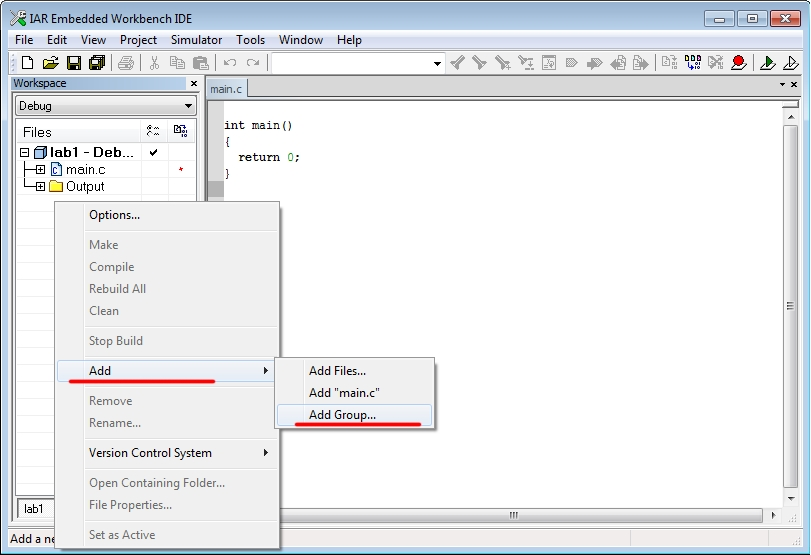
\includegraphics[scale=0.5]{Image/6.jpg}
\end{center}

\caption{Создание новой группы}
\end{figure}

Добавьте в созданные папки файлы библиотек \verb\stm32l1xx_gpio.h\, \verb\stm32l1xx_gpio.с\, \verb\stm32l1xx_rcc.c\, \verb\stm32l1xx_rcc.h\ из папки \verb\STM32L1xx_StdPeriph_Driver\.


\begin{figure}[h!]
\begin{center}
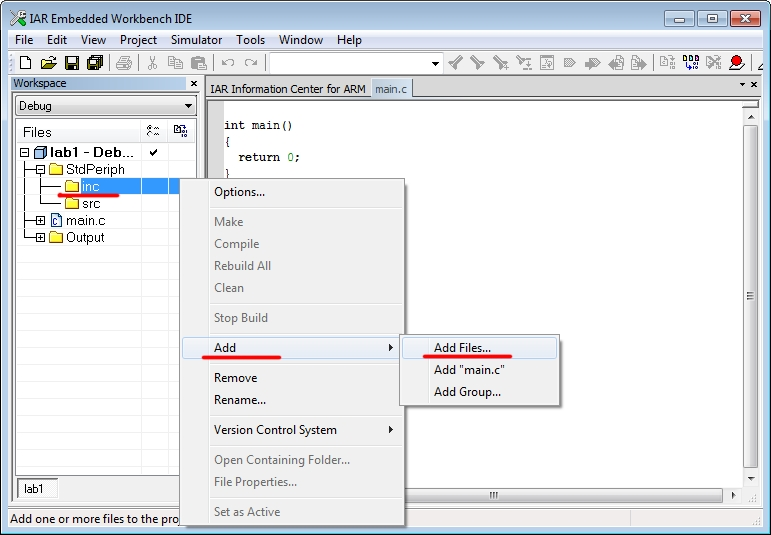
\includegraphics[scale=0.5]{Image/7.jpg}
\end{center}
\caption{Добавление файлов библиотек}
\end{figure}

Для дальнейшей работы необходимо настроить проект под заданный микроконтроллер.

\begin{figure}[h!]
\begin{center}
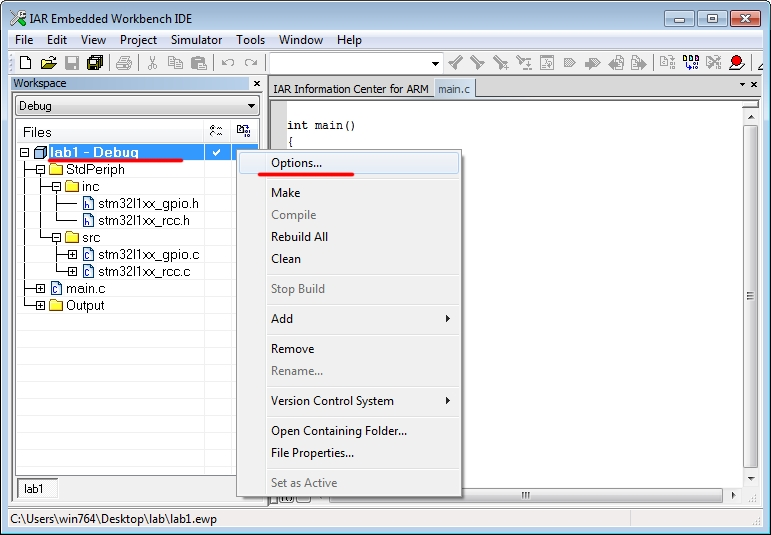
\includegraphics[scale=0.5]{Image/8.jpg}
\end{center}
\caption{Настройка проекта}
\end{figure}

В категории  \textit{ General Options}, во вкладке \textit{Target}, отметьте пункт \textit{Device} и в выпадающем списке выберите микроконтроллер 
\begin{center}
\textit{ST => ST ST32L52xB}
\end{center}

\begin{figure}[H]
\begin{center}
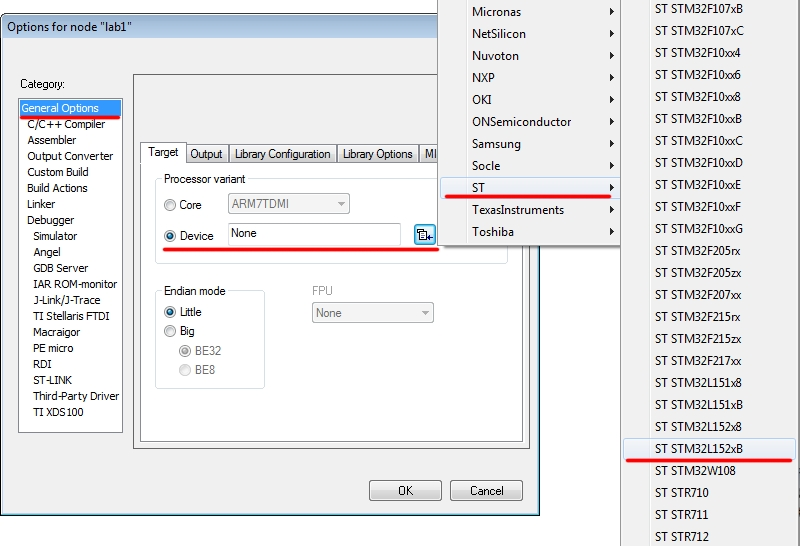
\includegraphics[scale=0.5]{Image/9.jpg}
\end{center}
\caption{Выбор микроконтроллера}
\end{figure}

В категории \textit{General Options}, во вкладке \textit{Library Configuration}, в выпадающем списке \textit{Library} выберите \textit{Full} -- для полного использования библиотеки времени выполнения (runtime library). Отметьте пункт \textit{Use CMSIS} для использования файлов описания ядра, разработанных IAR.


\begin{figure}[h!]
\begin{center}
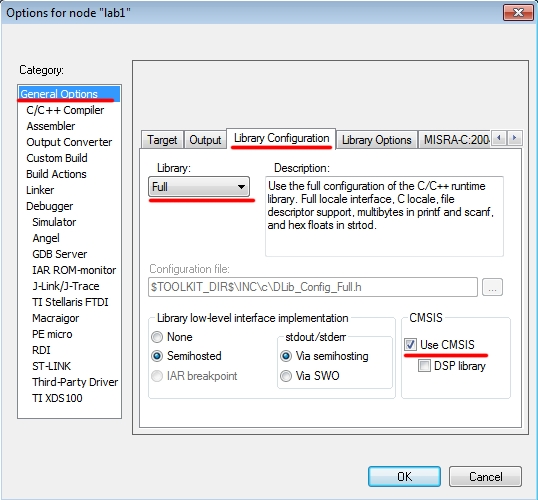
\includegraphics[scale=0.5]{Image/10.jpg}
\end{center}
\caption{Настройка библиотек}
\end{figure}

В категории  \textit{ C/C++ Compiler}, во вкладке \textit{Preprocessor} необходимо указать компилятору пути до заголовочных файлов.
Для относительного описания пути можно использовать переменную \verb\$PROJ_DIR$\ -- директория\ проекта.
\begin{verbatim}
$PROJ_DIR$\STM32L1xx_StdPeriph_Driver\inc
$PROJ_DIR$\CMSIS\CM3\DeviceSupport\ST\STM32L1xx
$PROJ_DIR$\
\end{verbatim}
Иногда принято размещать CMSIS и библиотеки переферии в одном месте, прописывая в настройках проекта абсолютный путь вида: \verb#C:\Library\CMSIS#, а не использовать локальную копию файлов библиотеки в каждом проекте.


\begin{figure}[H]
\begin{center}
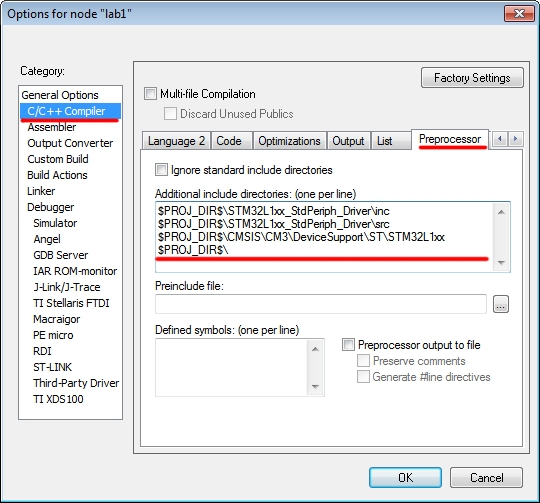
\includegraphics[scale=0.5]{Image/11.jpg}
\end{center}

\caption{казание дополнительных путей до файлов}
\end{figure}

По умолчанию IAR генерирует исполняемый файл в формате  \textit{ELF (Executable and Linkable Format)} -- формат исполняемых и компонуемых файлов, используемый во многих UNIX-подобных операционных системах. При желании, можно выбрать дополнительный формат. В категории  \textit{Output Converter} отметьте пункт  \textit{Generate additional output}, а в выпадающем списке  \textit{Output format} выберете  \textit{binary}.

\begin{figure}[H]
\begin{center}
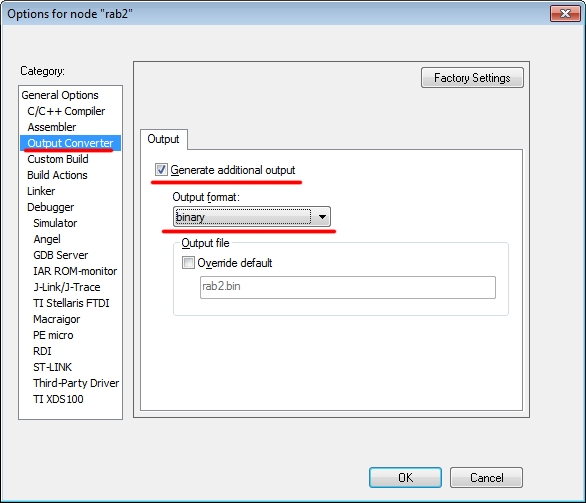
\includegraphics[scale=0.5]{Image/12.jpg}
\end{center}
\caption{Выбор формата исполняемого файла}
\end{figure}

В категории \textit{Linker}, отметьте пункт \textit{Override default} (отменить настройки по умолчанию), нажмите \textit{Edit} для настройки конфигурации компоновщика.


\begin{figure}[h!]
\begin{center}
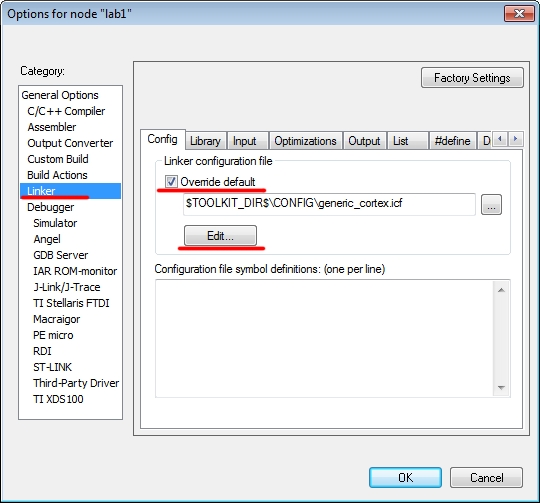
\includegraphics[scale=0.5]{Image/13.jpg}
\end{center}
\caption{Указание дополнительных путей до файлов}
\end{figure}

Во вкладке \textit{Vector Table} необходимо указать начало таблицы векторов прерываний. Адрес может быть \verb\0x00000000\ или \verb\0x08000000\. Адрес \verb\0x08000000\ указывает на начало внутренней Flash памяти, так же этот адрес рекомендует использовать STMicroelectronics в своем руководстве \textit{UM1451 User manual}. 


\begin{figure}[h!]
\begin{center}
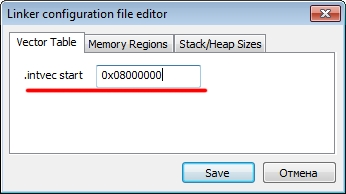
\includegraphics[scale=0.7]{Image/14.jpg}
\end{center}
\caption{Указание начала таблицы векторов прерываний}
\end{figure}

Во вкладке \textit{Memory Regions} задаются адреса начала и окончания ROM (ПЗУ) и RAM (ОЗУ). ROM -- внутренняя Flash память, начинается с адреса \verb\0х08000000\. Адрес окончания у каждого микроконтроллера разный и зависит от объема Flash памяти. Адрес окончания рассчитывается по формуле:

\begin{center}
	\[Адрес_{16} = адрес\ начала_{16} + размер\ Flash\ памяти_{16}-1_{16}\]
\end{center}

В микроконтроллере STM32L152RB 128 КБ Flash памяти, 16 КБ RAM.

\begin{center}
	\[0x08000000+(128\cdot1024)_{10}-1_{16}=0x0801FFFF\]
\end{center}

RAM память начинается с адреса \verb\0x20000000\. Адрес окончания рассчитывается аналогично:

\begin{center}
	\[0x20000000+(16\cdot1024)_{10}-1_{16}=0x20003FFF\]
\end{center}
STMicroelectronics, в своем руководстве \textit{UM1451 User manual}, рекомендует использовать адрес \verb\0x20004000\, т.е. \verb\0x20003FFF + 1\
\begin{figure}[H]
\begin{center}
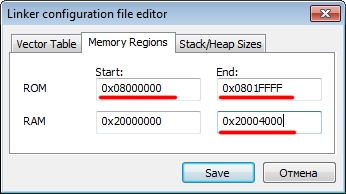
\includegraphics[scale=0.7]{Image/15.jpg}
\end{center}
\caption{Указание адреса начала и окончания ROM (ПЗУ) и RAM (ОЗУ)}
\end{figure}


В категории \textit{Debugger}, во вкладке \textit{Setup}, в выпадающем списке \textit{Driver} выберете \textit{ST-LINK}. Отметьте пункт \textit{Run to} и укажите значение \textit{main}, указывающее, что программа должна начинать работать с функции \textit{main}.



\begin{figure}[h!]
\begin{center}
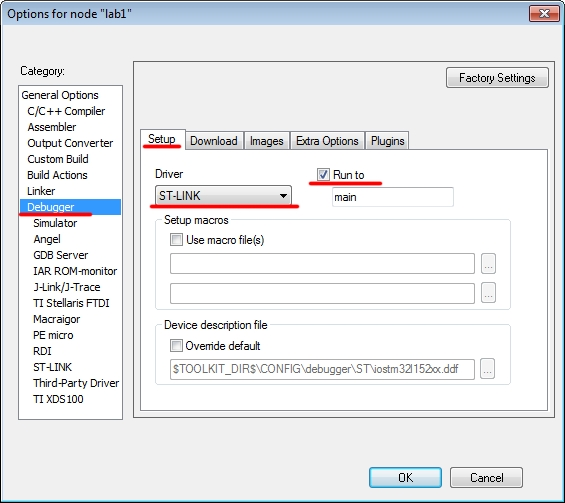
\includegraphics[scale=0.5]{Image/16.jpg}
\end{center}
\caption{Настройка отладчика. Часть 1}
\end{figure}

Во вкладке \textit{Download}, отметьте пункт \textit{Use flash loader(s)}, позволяющий программировать Flash непосредственно из среды IAR.


\begin{figure}[h!]
\begin{center}
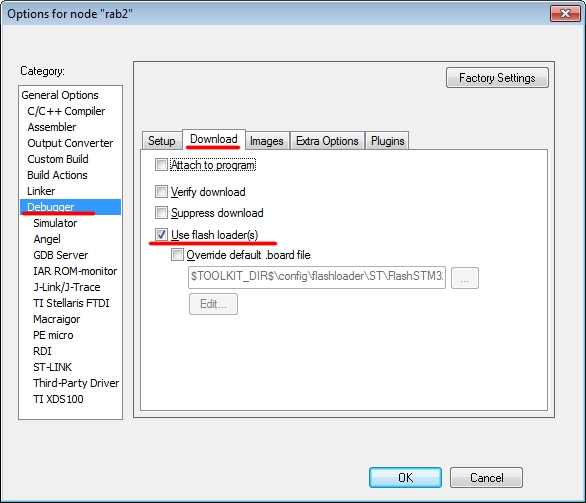
\includegraphics[scale=0.5]{Image/17.jpg}
\end{center}
\caption{Настройка отладчика. Часть 2}
\end{figure}

Для настройки встроенного программатора-отладчика\footnote{Программатор --- аппаратно-программное устройство, предназначенное для записи/считывания информации в постоянное запоминающее устройство} в категории \textit{ST-LINK}, в качестве интерфейса, выберете пункт \textit{SWD}.

\begin{figure}[h!]
\begin{center}
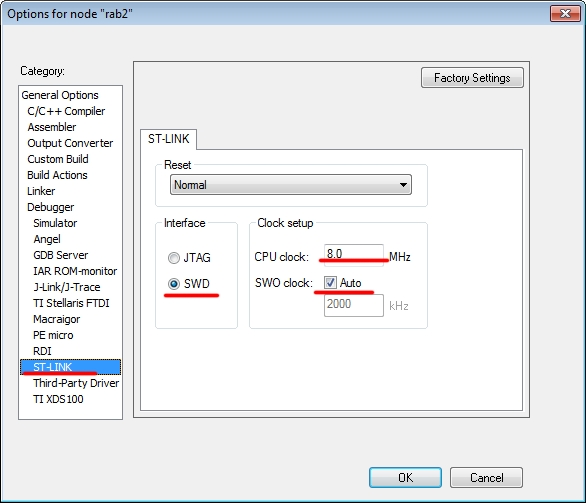
\includegraphics[scale=0.5]{Image/18.jpg}
\end{center}
\caption{Настройка программатора}
\end{figure}

При попытке собрать файлы проекта будет появляться ошибка:
\begin{verbatim}
Warning[Pe223]: function "assert_param" declared implicitly 
C:\EXAMPLES\lab1\stm32l1xx_gpio.c 124
\end{verbatim}

Ошибка указывает на то, что функция \textit{assert\_param()}, которая используется в библиотеке проверки своих аргументов, объявлена неявно. Для устранения ошибки создайте файл \verb\stm32l1xx_conf.h\ содержащий:

\begin{verbatim}
#ifndef STM32L1XX_CONF_H_
#define STM32L1XX_CONF_H_
/* ------------------- */
#ifndef USE_FULL_ASSERT
 #define assert_param(x)
#endif
/* ------------------- */
#endif
\end{verbatim}

Поместите файл в директорию проекта и добавьте его в проект. В исходные файлы подключаемых библиотек (\verb\stm32l1xx_rcc.c\, \verb\stm32l1xx_gpio.c\) добавьте строку:

\begin{verbatim}
#include <stm32l1xx_conf.h>
\end{verbatim}

Для сборки файлов проекта нажмите \textit{ Make} (F7). Будут созданы исполняемые файлы, в окне сообщений отобразиться количество ошибок и предупреждений.

\begin{figure}[H]
\begin{center}
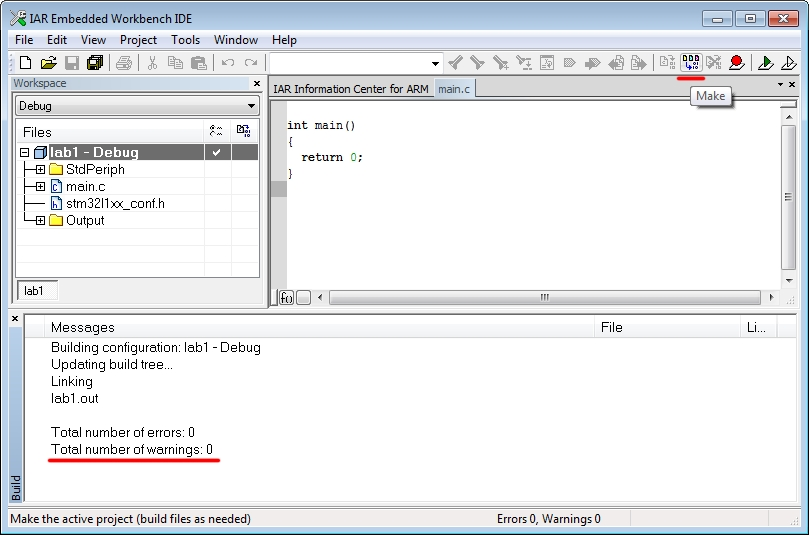
\includegraphics[scale=0.6]{Image/19.jpg}
\end{center}
\caption{Сборка файлов проекта}
\end{figure}


\subsection{Работа с периферией. Функции и структуры}
Для работы с периферией существуют два способа: Первый способ заключается в использовании регистров определенных в заголовочном файле \verb\stm32l1xx.h\ библиотеки CMSIS, расположенному в \verb#CMSIS/DeviceSupport/ST/STM32L1xx#. Для записи в регистр используются битмаски или шестнадцатеричные коды. Программирование через регистры достаточно трудно, но позволяет добиться большей производительности. Программирование с использованием регистров будет описано во второй лабораторной работе

Второй способ заключается в использовании готовых библиотек, например,\textit{ Standard Peripherals Library (SPL)} или \textit{Touch-Sensing Library (TSL)}. Библиотеки предоставляют готовые функции для работы с периферией, однако, скорость выполнения программы снижается, поскольку, в конечном итоге, все библиотечные функции управляют периферией через регистры. 

В данной лабораторной работе управление периферией (светодиодами) будет происходить через библиотеку \textit{Standard Peripherals Library (SPL)}, все необходимые для этого функции находятся в файлах \verb\stm32l1xx_gpio.h\, \verb\stm32l1xx_rcc.h\ в папке \verb#LabWorkSTM32L/Materials/STM32L1xx_StdPeriph_Driver#.

Светодиод \textit{LD3} подключен к порту ввода-вывода \textit{PB7}, светодиод \textit{LD4} подключен к порту ввода-вывода \textit{PB6}. По умолчанию периферия STM32 не работает, пока на нее не подан тактирующий сигнал. Для подачи тактирующего сигнала используется функция, прототип которой объявлен в заголовочном файле \verb\stm32l1xx_rcc.h\:
\begin{verbatim}
void RCC_AHBPeriphClockCmd(uint32_t RCC_AHBPeriph, 
                           FunctionalState NewState);
\end{verbatim}


Где \textit{AHB} --- шина, от которой происходит тактирование. Определить нужную шину можно по названию именованной константы в файле  \verb\stm32l1xx_rcc.h\:
\begin{verbatim}
...
#define RCC_AHBPeriph_GPIOA       RCC_AHBENR_GPIOAEN
#define RCC_AHBPeriph_GPIOB       RCC_AHBENR_GPIOBEN
#define RCC_AHBPeriph_GPIOC       RCC_AHBENR_GPIOCEN
#define RCC_AHBPeriph_GPIOD       RCC_AHBENR_GPIODEN
#define RCC_AHBPeriph_GPIOE       RCC_AHBENR_GPIOEEN
...
\end{verbatim}
Или на функциональной схеме, приведенной на рисунке 

\begin{Huge}
===================================

ФУНКЦИОНАЛЬНАЯ СХЕМА

===================================
\end{Huge}


В качестве первого аргумента функции используется приведенная выше именованная константа \verb\RCC_AHBPeriph_GPIOB\ (В случае портов PB6, PB7). В качестве второго аргумента используется константа перечисляемого типа \verb\ENABLE\ или \verb\DISABLE\, определенная в файле \verb\stm32l1xx.h\:

\begin{verbatim}
typedef enum {DISABLE = 0, ENABLE = !DISABLE} FunctionalState;
\end{verbatim}
Таким образом, функция для подачи тактирующего сигнала на порты GPIOB примет вид:
\begin{verbatim}
RCC_AHBPeriphClockCmd(RCC_AHBPeriph_GPIOB, ENABLE);
\end{verbatim}

Для описания режимов работы порта необходимо объявить переменную структурного типа \verb\GPIO_InitTypeDef\, которая содержит настройки порта в качестве полей структуры. Структура описывается в заголовочном файле периферии, которую необходимо инициализировать. В данной работе используются GPIO, следовательно, информация о структуре находиться в файле \verb\stm32l1xx_gpio.h\:
\begin{verbatim}
typedef struct
{
uint32_t GPIO_Pin;            /*!< Specifies the GPIO pins to be 						  
                              configured. This parameter can be any 					       
                              value of @ref GPIO_pins_define */

GPIOMode_TypeDef GPIO_Mode;   /*!< Specifies the operating mode for 						   
                              the selected pins. This parameter can 						   
                              be a value of @ref GPIOMode_TypeDef */

GPIOSpeed_TypeDef GPIO_Speed; /*!< Specifies the speed for the 						    
                              selected pins. This parameter can be a 					    
                              value of @ref GPIOSpeed_TypeDef */

GPIOOType_TypeDef GPIO_OType; /*!< Specifies the operating output 						    
                              type for the selected pins. This 						    
                              parameter can be a value of @ref 						    
                              GPIOOType_TypeDef */

GPIOPuPd_TypeDef GPIO_PuPd;   /*!< Specifies the operating Pull-						    
                              up/Pull down for the selected pins. 						    
                              This parameter can be a value of @ref 					    
                              GPIOPuPd_TypeDef */
}GPIO_InitTypeDef;
\end{verbatim}

Поля структуры имеют типы, определенные в качестве перечислений (enum) в файле \verb\stm32l1xx_gpio.h\:
\begin{verbatim}
typedef enum
{ 
  GPIO_Speed_400KHz = 0x00, /*!< Very Low Speed */
  GPIO_Speed_2MHz   = 0x01, /*!< Low Speed */
  GPIO_Speed_10MHz  = 0x02, /*!< Medium Speed */
  GPIO_Speed_40MHz  = 0x03  /*!< High Speed */
}GPIOSpeed_TypeDef;
...
typedef enum
{ 
  GPIO_Mode_IN   = 0x00, /*!< GPIO Input Mode */
  GPIO_Mode_OUT  = 0x01, /*!< GPIO Output Mode */
  GPIO_Mode_AF   = 0x02, /*!< GPIO Alternate functionMode */
  GPIO_Mode_AN   = 0x03  /*!< GPIO Analog Mode */
}GPIOMode_TypeDef;
...
\end{verbatim}
В данной работе структура будет иметь следующий вид:
\begin{verbatim}
GPIO_InitTypeDef Имя_структуры;
Имя_структуры.GPIO_Pin = GPIO_Pin_7 | GPIO_Pin_6 ; 
Имя_структуры.GPIO_Mode = GPIO_Mode_OUT;
Имя_структуры.GPIO_Speed = GPIO_Speed_2MHz;
Имя_структуры.GPIO_OType = GPIO_OType_PP;
\end{verbatim}

\verb\GPIO_Mode_OUT\ -- указывает, что порт является выходом. В случае если не указать тип в структуре, то при подаче питания на отладочную плату порт будет находиться в произвольном состоянии.

\verb\GPIO_OType_PP\ -- указывает, что выход имеет два состояния (Push-Pull) -- двухтактный полноценный выход или 0 или 1.

Для портов используется функция, прототип которой объявлен в заголовочном файле \verb\stm32l1xx_gpio.h\:
\begin{verbatim}
void GPIO_Init(GPIO_TypeDef* GPIOx, GPIO_InitTypeDef* GPIO_InitStruct);
\end{verbatim}
В качестве аргументов функции передаются указатель передаются порт и на сформированную структуру:
\begin{verbatim}
GPIO_Init(GPIOB, &Имя структуры);
\end{verbatim}
Для подачи питания на светодиод необходимо использовать функцию, прототип которой объявлен в заголовочном файле  \verb\stm32l1xx_gpio.h\:
\begin{verbatim}
void GPIO_SetBits(GPIO_TypeDef* GPIOx, uint16_t GPIO_Pin);
\end{verbatim}
В качестве аргументов функции передаются указатель на порт и именованная константа, определенная в заголовочном файле  \verb\stm32l1xx_gpio.h\, отвечающая за необходимый пин:
\begin{verbatim}
...
#define GPIO_Pin_2 ((uint16_t)0x0004)/*!< Pin 2 selected */
#define GPIO_Pin_3 ((uint16_t)0x0008)/*!< Pin 3 selected */
#define GPIO_Pin_4 ((uint16_t)0x0010)/*!< Pin 4 selected */
...
\end{verbatim}
Для того, что бы подать питания на светодиод LD3, подключенному к порту B, пину 7 (PB7), необходимо использовать функцию следующего вида:
\begin{verbatim}
GPIO_SetBits(GPIOB, GPIO_Pin_7);
\end{verbatim}
Что бы отключить питание используется функция с аналогичными аргументами:
\begin{verbatim}
void GPIO_ResetBits(GPIO_TypeDef* GPIOx, uint16_t GPIO_Pin);
\end{verbatim}
В качестве программной задержки между подачей питания и отключением питания используется цикл \textit{for} без инструкций:
\begin{verbatim}
for (int i = 0; i <= 100000; i++)
    ;
\end{verbatim}
Данный пример временной задержки является самым простым. В большинстве программ для генерации задержки используют таймеры.
\subsection{Загрузка программы в микроконтроллер и ее отладка}
После создание программы, нужно создать исполняемые файлы, для этого в главном меню выберите пункт 
\begin{center}
\textit{Project => Make}
\end{center}
или на панели инструментов\textit{ Make} (F7). При последующем изменении программы, инструмент \textit{Make} скомпилирует файлы, которые подверглись изменению с момента первоначального создания исполняемых файлов. Функция \textit{Compile} (Ctrl+F7) компилирует только выбранные файлы. 

\begin{figure}[h!]
\begin{center}
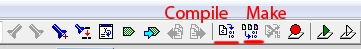
\includegraphics[scale=0.7]{Image/20.jpg}
\end{center}
\caption{Создание исполняемых файлов}
\end{figure}

Подключите отладочную плату STM32l-Discovery через разъем Mini USB к USB разъему компьютера. Для загрузки программы в микроконтроллер в главном меню выберите пункт 
\begin{center}
\textit{Project => Download and Debug}
\end{center}
или на панели инструментов \textit{Download and Debug} (Ctrl+D). 

 
\begin{figure}[h!]
\begin{center}
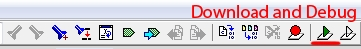
\includegraphics[scale=0.7]{Image/21.jpg}
\end{center}
\caption{Загрузка программы в микроконтроллер}
\end{figure}

После завершения загрузки программы в микроконтроллер, в IAR появиться панель отладки. 
\begin{figure}[h!]
\begin{center}
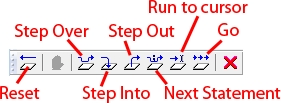
\includegraphics[scale=0.7]{Image/22.jpg}
\end{center}
\caption{Панель отладки}
\end{figure}

\textit{Step Over } -- выполняется следующая инструкция, оператор или функция, без входа в саму функцию.

\textit{Step Into } -- выполняется следующая инструкция, оператор или функция c входом в саму функцию.

\textit{Step Over } -- выполняется следующая инструкция, оператор или функция c выходом из функции.

\textit{Next Statement} -- выполняется следующая инструкция, оператор или функция без остановки вызовов функций.

\textit{Run to cursor} --  выполняется следующая инструкция, оператор или функция до выделенного фрагмента кода.

\textit{Reset} -- отладка выполняется с начала программы.

\textit{Go} -- выполняется следующая инструкция, оператор или функция до метки или окончания программы.

Для контроля значений переменных и функций используется инструмент \textit{Live Watch}. 
\begin{center}
\textit{View => Live Watch}
\end{center}
\textit{Live Watch} позволяет отслеживать значение выбранных переменных во время выполнения программы.
	Для запуска загруженной программы в микроконтроллер нажмите на панели отладки на \textit{Go} (F5).
	Все инструменты отладки дополнительно приведены в пункте \textit{Debug} в главном меню.




 
\section{Порядок выполнения лабораторной работы №1}
\begin{enumerate}
\item Выбрать вариант задания в приложении \ref{Lab1Var} в соответствии с номером в журнале. 
\item Создать в папке с номером группы на рабочем столе папку \verb#Lab1# для файлов проекта.
\item Скопировать в созданную папку \verb#Lab1#, папку CMSIS из папки \verb#LabWorkSTM32L/Materials# на рабочем столе.
\item Добавить в созданную папку с проектом папку \verb#STM32L1xx_StdPeriph_Driver# из папки \verb#LabWorkSTM32L/Materials#.
\item Добавить в созданную папку с проектом файл \verb\stm32l1xx_conf.h\ из папки \verb#LabWorkSTM32L/Materials#, добавить его в проект.
\item Добавьте в файлы \verb\stm32l1xx_gpio.c\, \verb\stm32l1xx_rcc.c\ строку:
\begin{verbatim}
#include <stm32l1xx_conf.h>
\end{verbatim}
\item Создать и настроить проект в среде разработки IAR. В качестве имени проекта указать \textit{lab1}, все файлы настроек проекта сохранить в папке \verb#Lab1#.
\item Добавить в проект IAR файлы \verb\stm32l1xx_gpio.c\, \verb\stm32l1xx_gpio.h\, \verb\stm32l1xx_rcc.c\, \verb\stm32l1xx_rcc.h\.
\item Построить блок-схему алгоритма главной программы.
\item Написать программу для микроконтроллера на языке Си.
\item Подключить отладочную плату STM32L-Discovery к компьютеру.
\item Загрузить программу в микроконтроллер и произвести ее отладку.
\item Отчет.
\end{enumerate}
\begin{huge}
Подумать над отчетом и интеграцией с гитом
\end{huge}


\section{Пример выполнения лабораторной работы №1}
Разработать программу для микроконтроллера в среде IAR и построить блок схему алгоритма главной программы. Работа светодиодов LD3 (Green) и LD4 (Blue) задается временными диаграммами. Последовательность, приведенная на временной диаграмме, должна повторяться бесконечно.
\begin{figure}[H]
\begin{center}
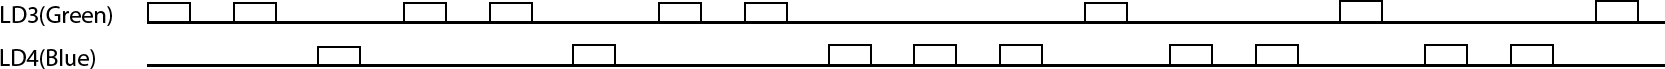
\includegraphics[scale=0.3]{Image/77.jpg} 
\end{center}
\caption{Временная диаграмма}
\end{figure}

\begin{figure}[H]
\begin{center}
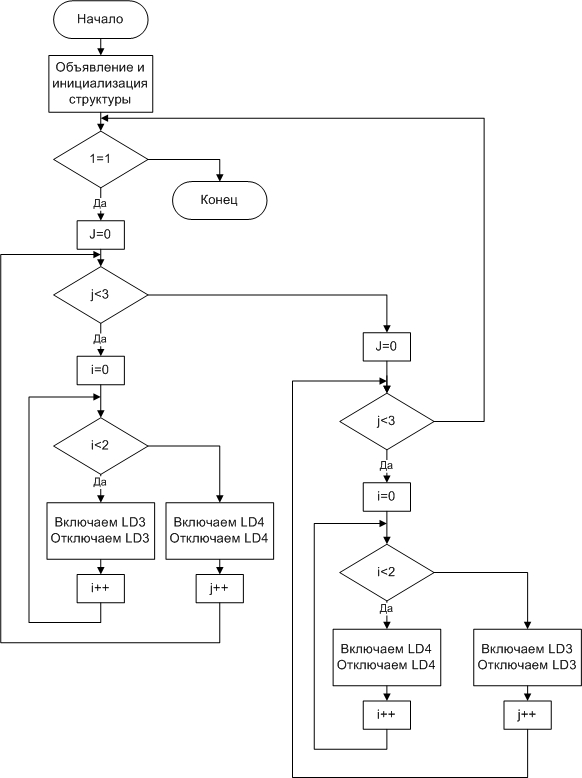
\includegraphics[scale=0.6]{Image/78.jpg} 
\end{center}
\caption{Схема алгоритма главной программы}
\end{figure}

\subsection{Пример главной программы для микроконтроллера}
\begin{verbatim}
#include <stm32l1xx.h>
#include <stm32l1xx_conf.h>
#include <stm32l1xx_gpio.h>
#include <stm32l1xx_rcc.h> 
void delay(int B); /*Прототип функции delay()*/
void led3(void);   /*Прототип функции led3()*/
void led4(void);   /*Прототип функции led4()*/

int main(void)
{
/*Объявление переменных типа uint32_t*/   
uint32_t i,j; 

/*Объявление структуры GPIO_InitStructure*/ 
GPIO_InitTypeDef GPIO_InitStructure; 
/*Включение тактирования*/
RCC_AHBPeriphClockCmd(RCC_AHBPeriph_GPIOB, ENABLE);   
GPIO_InitStructure.GPIO_Pin = GPIO_Pin_7 | GPIO_Pin_6 ;
GPIO_InitStructure.GPIO_Mode = GPIO_Mode_OUT;
GPIO_InitStructure.GPIO_Speed = GPIO_Speed_10MHz;
GPIO_InitStructure.GPIO_OType = GPIO_OType_PP;
/*Инициализация структуры*/        
GPIO_Init(GPIOB, &GPIO_InitStructure);  
  while (1)
  {
    j=0;
      while (j<3)
      {
        for (i=0;i<2;i++)
        led3();
        led4();
        j++;       
      }
    j=0;
      while (j<3)
     {
        for (i=0;i<2;i++)
        led4();
        led3();
        j++;       
      }         
  }
}
void delay(int B) /*Определение функции delay()*/
{
  int i;  
  for (i=0;i<=B;i++)
  ;
}
void led3(void)   /*Определение функции led3()*/
{
  GPIO_SetBits(GPIOB, GPIO_Pin_7);
  delay(100000);
  GPIO_ResetBits(GPIOB, GPIO_Pin_7);
  delay(100000);
}
void led4(void)   /*Определение функции led4()*/
{
  GPIO_SetBits(GPIOB, GPIO_Pin_6);
  delay(100000);
  GPIO_ResetBits(GPIOB, GPIO_Pin_6);
  delay(100000);
}
\end{verbatim}

\section{Варианты заданий к лабораторной работе №1}
\label{Lab1Var}
\begin{figure}[H]
\begin{center}
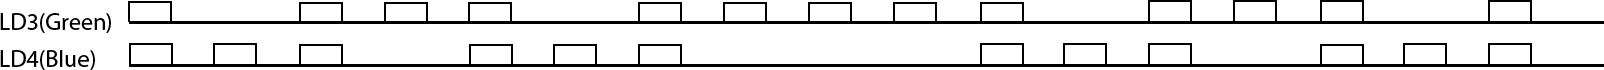
\includegraphics[scale=0.3]{Image/79.jpg} 
\end{center}
\caption{Вариант №1}
\end{figure}
\begin{figure}[H]
\begin{center}
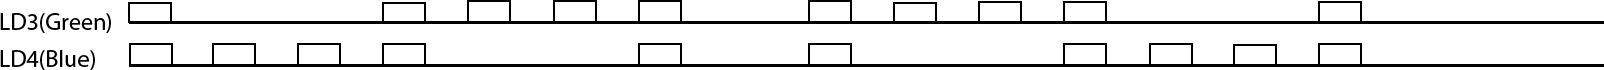
\includegraphics[scale=0.3]{Image/80.jpg} 
\end{center}
\caption{Вариант №2}
\end{figure}
\begin{figure}[H]
\begin{center}
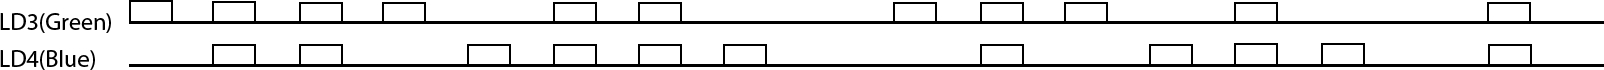
\includegraphics[scale=0.3]{Image/81.jpg} 
\end{center}
\caption{Вариант №3}
\end{figure}
\begin{figure}[H]
\begin{center}
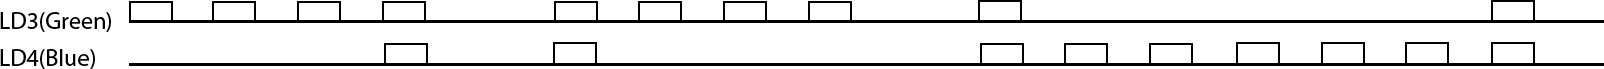
\includegraphics[scale=0.3]{Image/82.jpg} 
\end{center}
\caption{Вариант №4}
\end{figure}
\begin{figure}[H]
\begin{center}
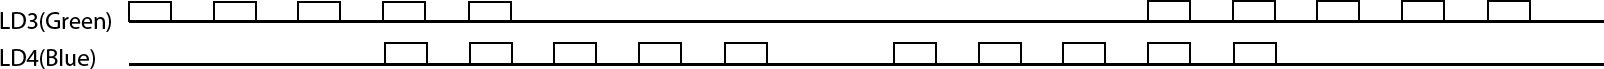
\includegraphics[scale=0.3]{Image/83.jpg} 
\end{center}
\caption{Вариант №5}
\end{figure}
\begin{figure}[H]
\begin{center}
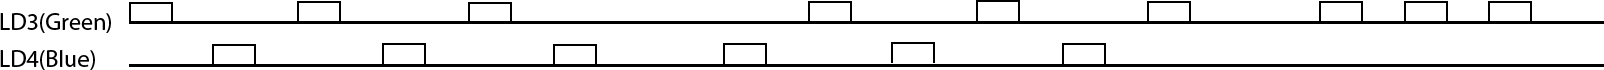
\includegraphics[scale=0.3]{Image/84.jpg} 
\end{center}
\caption{Вариант №6}
\end{figure}
\begin{figure}[H]
\begin{center}
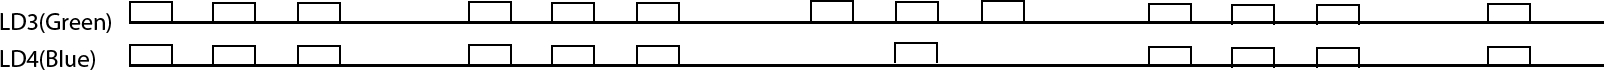
\includegraphics[scale=0.3]{Image/85.jpg} 
\end{center}
\caption{Вариант №7}
\end{figure}
\begin{figure}[H]
\begin{center}
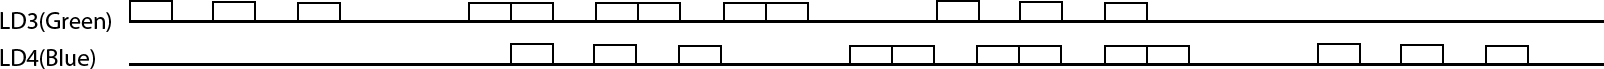
\includegraphics[scale=0.3]{Image/86.jpg} 
\end{center}
\caption{Вариант №8}
\end{figure}
\begin{figure}[H]
\begin{center}
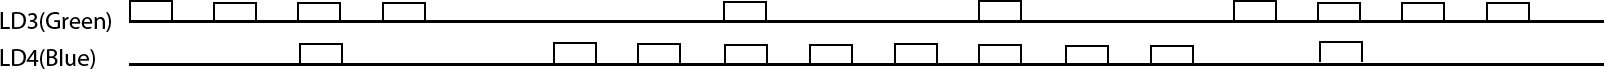
\includegraphics[scale=0.3]{Image/87.jpg} 
\end{center}
\caption{Вариант №9}
\end{figure}
\end{document}
